% Fra forsiden: CLRS refererer til 4. udgave; nogle opgaver henviser til online-kapitler fra 3. udgave, som ikke er med i 4. udgave.
\section*{Multiple-choice}\label{sec:mc}

Dine svar skal indtastes i ITX-systemets multiple-choice modul.

\multiplechoicestart


\spoergsmaal{Sortering}
Betragt en variant af {\sc Merge-Sort} der deler input op i \emph{tre} dele, der er lige store (op til afrunding), sorterer hver del rekursivt, og derefter fletter de tre dele sammen med to kald til {\sc Merge} (CLRS sektion 2.3). Pseudokoden ser således ud:
\begin{codebox}
  \Procname{$\proc{Merge3-Sort}(A, p, s)$}
  \li \If $p<s$ \Do
  \li $q = \lfloor (2\cdot p+ s)/3\rfloor$
  \li $r = \lfloor (p+2\cdot s)/3\rfloor$
  \li $\proc{Merge3-Sort}(A, p, q)$
  \li $\proc{Merge3-Sort}(A, q+1, r)$
  \li $\proc{Merge3-Sort}(A, r+1, s)$
  \li $\proc{Merge}(A, p, q, r)$
  \li $\proc{Merge}(A, p, r, s)$ \End
\end{codebox}

\noindent
Hvilken rekursionsligning beskriver køretiden $T(n)$ af $\proc{Merge3-Sort}$ på et input af størrelse~$n$ (hvor $n = s - p + 1$)?
\etsvar
\mulighederstart
\svar $T(n) = T(n/2) + \Theta(n)$
\svar $T(n) = T(2n/3) + \Theta(n)$
\svar $T(n) = 2\cdot T(n/3) + \Theta(n)$
\svar $T(n) = 2\cdot T(2n/3) + \Theta(n)$
\svar $T(n) = 3\cdot T(n/2) + \Theta(n)$
\svar $T(n) = 3\cdot T(n/3) + \Theta(n)$ \korrekt
\mulighederslut

\forklaring{De tre rekursive kald tager hver tid $T(n/3)$ mens de to kald til {\sc Merge} tager samlet tid $\Theta(n)$.}




\spoergsmaal{Rekursionsligninger}
Hvilken af nedenstående rekursionsligninger, nummereret $i=1,\dots,6$, har en løsning $T_i$ hvor $T_i(n) = O(n^2)$?
Antag at $T_i(n) = 1$ for $n\leq 1$. \fleresvar

\medskip\noindent
{\bf Eksempler.} Hvis $T_0(n) = \Theta(n)$ gælder også $T_0(n) = O(n^2)$. Hvis $T_0(n) = \Theta(2^n)$ gælder \emph{ikke} $T_0(n) = O(n^2)$.

\mulighederstart
\svar $T_1(n) = T_1(n/2) + \Theta(n^2)$ \korrekt
\svar $T_2(n) = 4\cdot T_2(n/2) + \Theta(n^2)$
\svar $T_3(n) = 3\cdot T_3(n/2) + \Theta(n)$  \korrekt
\svar $T_4(n) = T_4(n/3) + \Theta(n)$ \korrekt
\svar $T_5(n) = 2\cdot T_5(n/3) + \Theta(n)$ \korrekt
\svar $T_6(n) = 2\cdot T_6(n-2) + \Theta(n)$
\mulighederslut

\forklaring{Rekursionsligning 1--5 kan løses med master theorem og har løsninger henholdsvis $T_1(n)=\Theta(n^2)$, $T_2(n)=\Theta(n^2\lg n)$, $T_3(n)=\Theta(n^{\lg_2 3})$, $T_4(n)=\Theta(n)$, og $T_5(n)=\Theta(n)$. Rekursionsligning 6 kan løses som $T_6(n)=\Theta(2^{n/2})$ ved hjælp af substitutionsmetoden.}




\spoergsmaal{Nedre grænser for sortering}
{\sc Merge-Sort} og (deterministisk) {\sc Quicksort} som beskrevet i CLRS sektion 2.3 og 7.1 er eksempler på sammenligningsbaserede sorteringsalgoritmer (\emph{eng., comparison sort algorithms}).
Hvilke konklusioner kan drages som følge af den nedre grænse for sortering, Theorem 8.1 i CLRS?
(Du skal ikke tage stilling til om konklusionen er sand, blot om den er en logisk konsekvens af Theorem~8.1.)
\fleresvar
\mulighederstart
\svar Der findes et input hvor {\sc Quicksort} kører i tid $O(n \lg n)$ i værste fald
\svar Der findes et input hvor {\sc Merge-Sort} kører i tid $O(n \lg n)$ i værste fald
\svar Der findes et input hvor {\sc Quicksort} kører i tid $\Omega(n \lg n)$ i værste fald \korrekt
\svar Der findes et input hvor {\sc Merge-Sort} kører i tid $\Omega(n \lg n)$ i værste fald \korrekt
\svar I gennemsnit over alle input kører {\sc Merge-Sort} i tid $\Omega(n \lg n)$
\svar I gennemsnit over alle input kører {\sc Quicksort} i tid $O(n \lg n)$
\mulighederslut

\forklaring{Theorem 8.1 giver ikke nogen $O(n \lg n)$ øvre grænse på antal sammenligninger (og en sådan grænse findes ikke, da der jo eksisterer langsommere sorteringsalgoritmer). Det udelukker svar 1, 2 og 6. Derimod udtaler Theorem 8.1 sig om tiden for det værste input for såvel {\sc Merge-Sort} som {\sc Quicksort}. Svarmulighed 5 er et korrekt udsagn, men det er ikke en konsekvens af Theorem 8.1, der kun udtaler sig om værste fald. }





\spoergsmaal{Løkkeinvarianter}
Betragt følgende funktion, i pseudo-kode notationen fra CLRS, hvor input $A$ er et array af reelle tal og $n$ er længden af $A$.
\begin{codebox}
  \Procname{$\proc{Variance}(A, n)$}
  \li $r = 0$
  \li $s = 0$
  \li \For $i = 1$ \To $n$
  \li \Do $r = r + A[i] \cdot A[i]$
  \li $s = s + A[i]$ \End
  \li \Return $r / n - (s\cdot s)/(n\cdot n)$
\end{codebox}

{\bf Eksempel:} For $n=4$ og $A = \langle\frac{1}{2},2,0,-\frac{1}{2}\rangle$ returnerer {\sc Variance} værdien $7/8$.
\medskip

\noindent
Hvilke udsagn er gyldige invarianter, der er sande efter udførelsen af linje 5 i {\bf for}-løkken?
\fleresvar
\mulighederstart
\svar $s\leq r$
\svar $s\geq 0$
\svar $r\geq 0$ \korrekt
\svar $i\geq 0$ \korrekt
\svar $s = \sum_{j=1}^n A[j]$
\svar $r = \sum_{j=1}^i A[j]^2$ \korrekt
\svar $i \leq n$ \korrekt
\mulighederslut

\forklaring{ Udsagn 1 gælder ikke efter 1 iteration hvis $A[1]=1/2$. Udsagn 2 gælder ikke efter 1 iteration hvis $A[1]=-1/2$. Udsagn 6 gælder per induktion pga.~initialiseringen af $r=0$ og da $r$ øger sin værdi med $A[i]^2$ i iteration $i$. Fordi $A[i] \cdot A[i]\geq 0$ medfører det at udsagn 3 er korrekt. Udsagn 5 gælder efter den sidste iteration, men er ikke en invariant. Udsagn 4 og 7 er invarianter da løkken starter med $i=1$ og terminerer når $i=n$.}




\spoergsmaal{Invarianter for dynamiske tabeller}
Betragt dynamiske tabeller (\emph{eng., dynamic tables}) som beskrevet i CLRS sektion 16.4.1, altså versionen \emph{uden} en {\sc Table-Delete} operation.
Hvilke af følgende er gyldige invarianter for algoritmen efter hver {\sc Table-Insert} operation?
\fleresvar
\mulighederstart
\svar $T.size = 0$
\svar $T.size \leq T.num$
\svar $T.size \leq 2\cdot T.num$ \korrekt
\svar $T.num = T.size$
\svar $T.num \leq T.size$ \korrekt
\svar $T.num \leq 2\cdot T.size$ \korrekt
\mulighederslut

\forklaring{
Udsagn 1 og 4 er betingelser der evalueres i {\sc Table-Insert} og ikke invarianter. Udsagn 5 er en invariant fordi den gælder initielt (når $T.size = 0$)og fordi $T.size$ fordobles når $T.size = T.num$, inden værdien af $T.num$ øges. Dette medfører at udsagn 6 også er sandt. Udsagn 2 er forkert og gælder fx ikke efter den anden fordobling når $T.size = 4$ og $T.num = 3$. Udsagn 3 gælder fordi det er sandt efter den første indsættelse ($T.num = T.size = 1$), og da $T.size$ kun fordobles når $T.num = T.size$, mens $T.size$ aldrig bliver mindre (fordi vi ikke har {\sc Table-Delete}).
}



\spoergsmaal{Amortiseret analyse}
Betragt dynamiske tabeller (\emph{eng., dynamic tables}) som beskrevet i CLRS sektion 16.4.2, altså versionen \emph{med} en {\sc Table-Delete} operation.
Vi betragter potentialfunktionen defineret i CLRS ligning (16.5), hvor $\alpha(T) = T.num / T.size$:
\[
\Phi(T) =
\begin{cases}
    2(T.num - T.size/2) \text{ if } \alpha(T) \geq 1/2,\\
    T.size - T.num \text{ if } \alpha(T) < 1/2 \enspace .
\end{cases}
\]
Hvilke af følgende udsagn er sande?
\fleresvar
\mulighederstart
\svar En {\sc Table-Insert} operation øger altid værdien af $\Phi(T)$
\svar En {\sc Table-Delete} operation øger altid værdien af $\Phi(T)$
\svar En {\sc Table-Insert} operation mindsker altid værdien af $\Phi(T)$
\svar En {\sc Table-Delete} operation mindsker altid værdien af $\Phi(T)$
\svar Værdien af $\Phi(T)$ er altid større eller lig med nul \korrekt
\svar Værdien af $\Phi(T)$ er altid mindre end eller lig med $T.size$ \korrekt
\mulighederslut

\forklaring{
Udsagn 1-4 er falske fordi effekten på potentialet af en operation afhænger af $\alpha(T)$, med en mindskning i det ene tilfælde og en øgning i det andet tilfælde. Udsagn 5 er sandt da $2 T.num \geq T.size \geq T.num$. Udsagn 6 er sandt da $2(T.num - T.size/2) \leq 2(T.size - T.size/2) = T.size$.
}



\spoergsmaal{Fibonaccihobe}\label{spm:fibonacci}
Denne opgave omhandler Fibonaccihobe (\emph{eng., Fibonacci heaps}) som beskrevet i CLRS digitalt kapitel 19 (dvs.~min-heap ordnede).
Som i CLRS figur 19.2.a illustreres rodlisten med stiplede linjer og markerede knuder tegnes med sort.
Hvilke nøgler er mulige på mindst én af knuderne markeret med spørgsmålstegn? \fleresvar

\begin{center}
  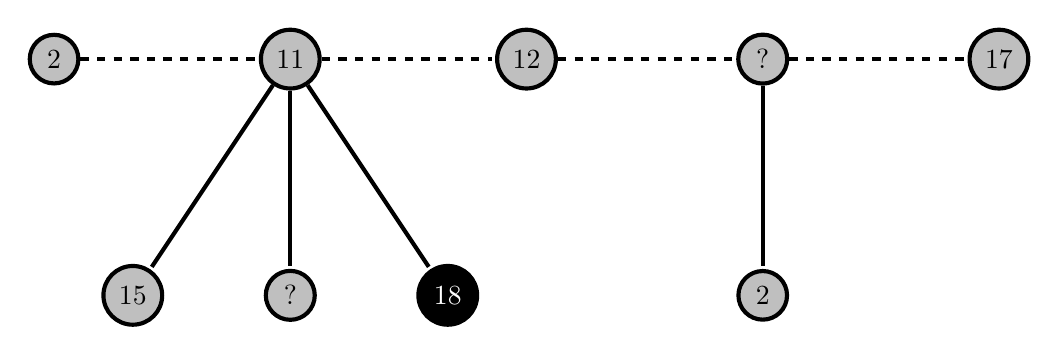
\begin{tikzpicture}[-,>=stealth,shorten >=1pt,auto,
      main node/.style={circle,draw}, line width=1.5pt]
  \node[main node,fill=lightgray] (a) at (0,0) {2};
  \node[main node,fill=lightgray] (b) at (3,0) {11};
  \node[main node,fill=lightgray] (f) at (1,-3) {15};
  \node[main node,fill=lightgray] (g) at (3,-3) {?};
  \node[main node,fill=black,text=white] (h) at (5,-3) {18};
  \node[main node,fill=lightgray] (c) at (6,0) {12};
  \node[main node,fill=lightgray] (d) at (9,0) {?};
  \node[main node,fill=lightgray] (i) at (9,-3) {2};
  \node[main node,fill=lightgray] (e) at (12,0) {17};
  \path[every node/.style={font=\small}]
  (a) edge[dashed] (b)
  (b) edge[dashed] (c)
  (c) edge[dashed] (d)
  (d) edge[dashed] (e)
  (b) edge (f)
  (b) edge (g)
  (b) edge (h)
  (d) edge (i)
  ;
  \end{tikzpicture}
  \end{center}
  
\mulighederstart
\svar 2 \korrekt
\svar 6
\svar 10
\svar 14 \korrekt
\svar 18 \korrekt
\svar 22 \korrekt
\mulighederslut

\forklaring{
Knuderne skal overholde min-heap egenskaben, dvs.~den ukendte knude til venstre skal indeholde en værdi som er større end eller lig med forældreknuden 11, og den ukendte knude til højre skal indeholde en værdi som er mindre end eller lig med dens børns værdier, dvs.~2. Derfor er 6 og 10 de eneste værdier, der ikke passer i nogen af knuderne.
}



\spoergsmaal{Tidskompleksitet for Fibonaccihobe}
Antag at der laves en {\sc Fib-Heap-Extract-Min} operation på en Fibonaccihob $H$(\emph{eng., Fibonacci heap}) med $n$ nøgler som beskrevet i CLRS digitalt kapitel 19.
Før operationen har potentialfunktionen værdien $\Phi(H)$ og efter operationen har den værdien $\Phi(H')$, hvor $H'$ er den nye Fibonaccihob.
Hvad kan vi med sikkerhed sige om tidsforbruget af {\sc Fib-Heap-Extract-Min} operationen der omdanner $H$ til $H'$?
\fleresvar

\mulighederstart
\svar Tiden er $O(n)$ \korrekt
\svar Tiden er $O(\lg n)$
\svar Tiden er $O(\lg n + \Phi(H) - \Phi(H'))$ \korrekt
\svar Tiden er $O(1 + \Phi(H) - \Phi(H'))$
\svar Tiden er $O(1)$
\mulighederslut

\forklaring{Den amortiserede analyse i CLRS viser at tidsforbruget er højst (en konstant gange med) $\lg n + \Phi(H) - \Phi(H')$. Da $0\leq \Phi(H) \leq n$ medfører det en tidsgrænse på $O(n)$, dvs.~svarmulighed 1 og 3 er korrekte. Svarmulighed 2 og 5 er ikke korrekte hvis rodlisten er længere end $O(\lg n)$, hvilket kan ske efter en række indsættelser, da {\sc Consolidate} løber igennem rodlisten. Svarmulighed 4 er ikke korrekt hvis der er en knude af grad $\lg n$ i rodlisten, da {\sc Consolidate} bruger tid proportionalt med graden, men ikke nødvendigvis mindsker potentialet. }






\spoergsmaal{Stavudskæring}
Betragt algoritmen \textsc{Extended-Bottom-Up-Cut-Rod}, CLRS sektion 14.1, side 372.
Lad $n=6$ og $p=\langle
4, 4, 13, 40, 43, 49\rangle$.
Hvilke arrays $r$ og $s$ returnerer algoritmen når den kaldes på input $(p,n)$?
\etsvar
\mulighederstart
\svar $r=\langle 0, 4, 8, 13, 40, 44, 48\rangle$ og $s=\langle 1, 1, 3, 4, 1, 4\rangle$
\svar $r=\langle 0, 4, 8, 13, 40, 44, 48\rangle$ og $s=\langle 1, 1, 3, 4, 1, 6\rangle$
\svar $r=\langle 0, 4, 8, 13, 40, 44, 49\rangle$ og $s=\langle 1, 1, 3, 4, 1, 4\rangle$
\svar $r=\langle 0, 4, 8, 13, 40, 44, 49\rangle$ og $s=\langle 1, 1, 3, 4, 1, 6\rangle$ \korrekt
%\svar $r=\langle 0, 4, 4, 13, 40, 43, 49\rangle$ og $s=\langle 1, 2, 3, 4, 5, 6\rangle$.
\mulighederslut
\forklaring{Ses ved at håndkøre algoritmen.}



\spoergsmaal{Paradigmer}
Betragt følgende pseudokode, der tager et array $A$ og to indekser $p$, $r$ som parametre.
%
\begin{codebox}
  \Procname{$\proc{MyAlgorithm}(A, p, r)$}
  \li \If $p<r$ \Do
  \li $q = \lfloor (p+ r)/2\rfloor$
  \li $x = \proc{MyAlgorithm}(A, p, q)$
  \li $y = \proc{MyAlgorithm}(A, q+1, r)$
  \li $z = \proc{MyAlgorithm}(A, p+1, r)$
  \li \Return $x+y+z$ \End
  \li \Else\Do
  \li \Return $A[p]$ \End
\end{codebox}
%
Hvilket af nedenstående paradigmer beskriver bedst $\proc{MyAlgorithm}$?
\etsvar
\mulighederstart
\svar Del og kombiner (eng.~\emph{divide and conquer}) \korrekt
\svar Dynamisk programmering (eng.~\emph{dynamic programming})
\svar Grådige algoritmer (eng.~\emph{greedy algorithms})
\mulighederslut
\forklaring{Algoritmen virker ved at kalde sig selv rekursivt på tre mindre probleminstanser og derefter kombinere resultaterne. Den bruger derfor del og kombiner. Der gemmes ikke nogen resultater, så koden bruger ikke dynamisk programmering. Der foregår heller ikke noget grådigt valg (ingen betingelser afhænger af indholdet i $A$), så det passer heller ikke godt med en grådig algoritme. }



%\newpage

\spoergsmaal{Huffman-koder}
Betragt bogstaverne a, b, c, d, e, f og tilhørende frekvenser a:13, b:5, c:7, d:9, e:6, f:8.
Vi kører Huffmans algoritme på frekvenserne, som beskrevet i CLRS afsnit 15.3.
Hvilket træ får vi som resultat?
\etsvar
\mulighederstart
\svar \qquad \includegraphics[page=6,valign=c]{ad-problems-2024-april-figs.pdf}
\itxsvar{Træ 1}
\svar \qquad \includegraphics[page=4,valign=c]{ad-problems-2024-april-figs.pdf}
\itxsvar{Træ 2}
\svar \qquad \includegraphics[page=5,valign=c]{ad-problems-2024-april-figs.pdf}
\itxsvar{Træ 3}
\svar \qquad \includegraphics[page=3,valign=c]{ad-problems-2024-april-figs.pdf} \korrekt
\itxsvar{Træ 4}
\svar \qquad \includegraphics[page=7,valign=c]{ad-problems-2024-april-figs.pdf}
\itxsvar{Træ 5}
\mulighederslut
\forklaring{Ses ved at håndkøre algoritmen.}





\spoergsmaal{Rød-sorte søgetræer}\label{q:red-black}
Betragt et rød-sort binært søgetræ $T$ (eng.~\emph{red-black binary search tree}), som beskrevet i CLRS kapitel 13.
Betragt nedenstående træ, hvor alle blade er udeladt (som på CLRS figur 13.1.c) og tre indre knuder er uspecificerede:

\begin{center}
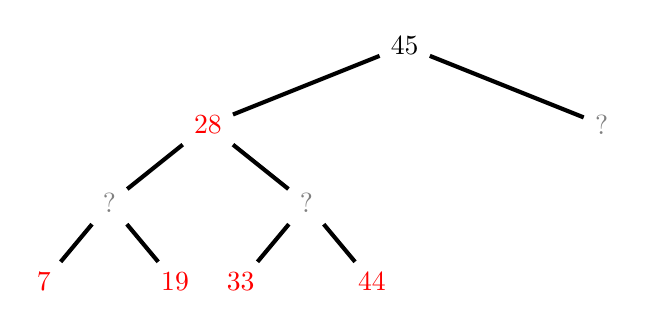
\begin{tikzpicture}[-,>=stealth,level/.style={sibling distance = 5cm/#1,
    level distance = 1cm}, line width=1.5pt] 
  \node [black] {45}
      child{ node [red] {28} 
              child{ node [gray] {?} 
                  child{ node [red] {7} }
                  child{ node [red] {19}}
              }
              child{ node [gray] {?}
                              child{ node [red] {33}}
                              child{ node [red] {44}}
              }                            
      }
      child{ node [gray] {?}
          }
  ; 
  \end{tikzpicture}  
\end{center}

\medskip

Hvilke knuder er mulige på mindst én af positionerne markeret med ?, hvis træet skal overholde invarianterne for et rød-sort binært søgetræ?
\fleresvar
\mulighederstart
\svar En rød knude med nøglen 13
\svar En sort knude med nøglen 17 \korrekt
\svar En rød knude med nøglen 29
\svar En sort knude med nøglen 37 \korrekt
\svar En rød knude med nøglen 48
\svar En sort knude med nøglen 84 \korrekt
\mulighederslut
\forklaring{ Alle de markerede knuder skal være sorte. De to til venstre fordi deres forælder er rød. Den sidste fordi der skal være lige mange sorte knuder på alle stier fra roden til bladene. Nøglerne 17, 37 og 84 er alle konsistente med invarianten at træet er et søgetræ (17 ligger mellem 7 og 19, 37 mellem 33 og 44, 84 er større end 45).
}



\spoergsmaal{Rotationer i rød-sorte søgetræer}
Betragt dette rød-sorte binære søgetræ $T$ (eng.~\emph{red-black binary search tree}), hvor bladene er udeladt på tegningen:
%
\begin{center}
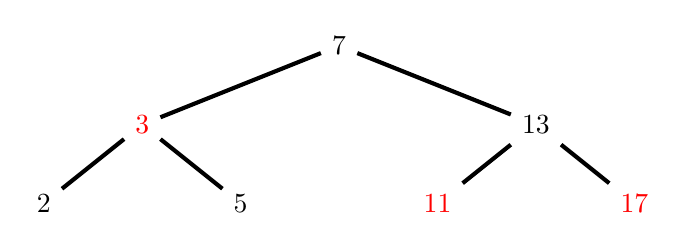
\begin{tikzpicture}[-,>=stealth,level/.style={sibling distance = 5cm/#1,
    level distance = 1cm}, line width=1.5pt] 
  \node [black] {7}
      child{ node [red] {3} 
              child{ node [black] {2} 
              }
              child{ node [black] {5}
              }                            
      }
      child{ node [black] {13}
              child{ node [red] {11} 
              }
              child{ node [red] {17}
              }
          }
  ; 
  \end{tikzpicture}  
\end{center}

\medskip

Antag at vi kører algoritmen {\sc Left-Rotate$(T,7)$} beskrevet i CLRS kapitel 13.2, altså med knuden $7$ som input.
Hvad sker med træet $T$?
\fleresvar
\mulighederstart
\svar 3 bliver den nye rodknude og farves sort
\svar 13 bliver den nye rodknude \korrekt
\svar Højden forbliver den samme
\svar Højden stiger med 1 \korrekt
\mulighederslut
\forklaring{ {\sc Left-Rotate$(T,7)$} gør 13 til rod med 7 og 17 under sig. Knude 11 bliver højre barn til 7. Ingen knuder skifter farve. Efter rotationen er knude 2 og 5 et skridt længere væk fra roden end inden.
}


\spoergsmaal{Mindste udspændende træ}
Betragt mindste udspændende træ (eng.~\emph{minimum spanning tree}) problemet på denne graf:
\begin{center}
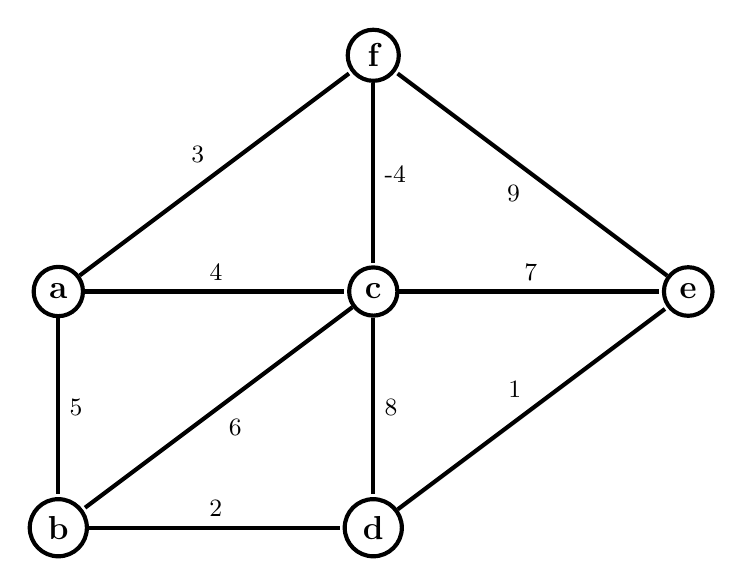
\begin{tikzpicture}[-,>=stealth,shorten >=1pt,auto,
  main node/.style={circle,draw,font=\large\bfseries}, line width=1.5pt]
\node[main node] (a) at (2,1.5) {a};
\node[main node] (b) at (2,-1.5) {b};
\node[main node] (c) at (6,1.5) {c};
\node[main node] (d) at (6,-1.5) {d};
\node[main node] (e) at (10,1.5) {e};
\node[main node] (f) at (6,4.5) {f};

\path[every node/.style={font=\small}]
(a) edge node {5} (b) 
edge node {4} (c)
(b) edge node {2} (d)
(a) edge node {3} (f)
(c) edge node {8} (d) 
edge node {7} (e) 
edge node {6} (b) 
(d) edge node {1} (e)
(e) edge node {9} (f) 
(f) edge node {-4} (c); 
\end{tikzpicture}
\end{center}
Hvilke kanter er med i det mindste udspændende træ (som er unikt)?
\fleresvar
\mulighederstart
\svar \{a,b\} \korrekt
\svar \{a,c\} 
\svar \{a,f\} \korrekt
\svar \{b,c\} 
\svar \{b,d\} \korrekt
\svar \{c,d\} 
\svar \{c,e\} 
\svar \{c,f\} \korrekt
\svar \{d,e\} \korrekt
\svar \{e,f\}
\mulighederslut
\forklaring{Mindste udspændende træ kan findes ved at køre fx Kruskal's eller Prim's algoritme. Kruskal's algoritme tilføjer kanterne i vægtrækkefølge, dvs.~starter med \{c,f\}, \{d,e\}, \{b,d\}, \{a,f\}, springer over \{a,c\} fordi det ville skabe en kreds, og afslutter med \{a,b\}. }



\spoergsmaal{Snit og sikre kanter}
Betragt følgende ikke-orienterede, vægtede og sammenhængende graf $G=(V,E)$ med knudemængden $V = \{A,B,C,D,E,F\}$: 
Vi er interesserede i lette kanter (eng.~\emph{light edges}) for en kantmængde $K$ i forskellige snit (eng.~\emph{cuts}).
Hvilke af følgende udsagn er sande for kantmængden $K = \{\{D,F\},\{C,E\},\{A,B\}\}$? \fleresvar

\begin{center}
  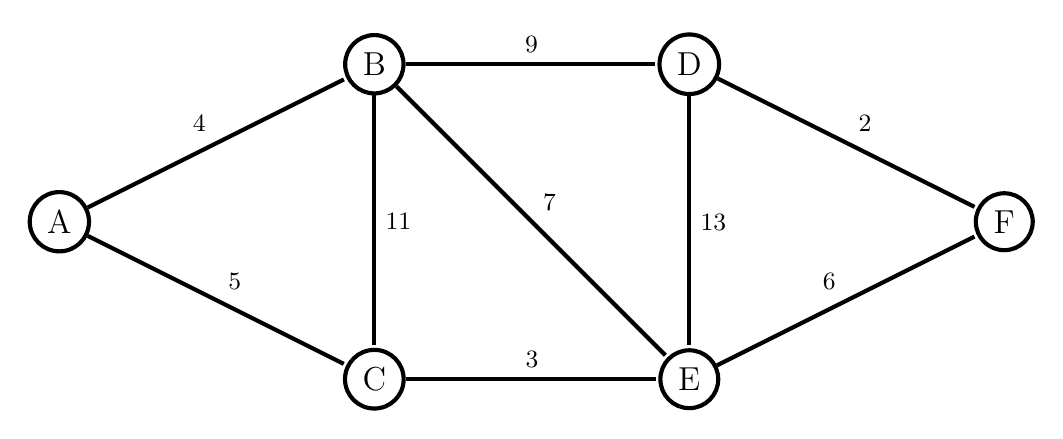
\begin{tikzpicture}[-,>=stealth,shorten >=1pt,auto,
      main node/.style={circle,draw,font=\large}, line width=1.5pt]
  \node[main node] (a) at (0,0) {A};
  \node[main node] (b) at (4,2) {B};
  \node[main node] (c) at (4,-2) {C};
  \node[main node] (d) at (8,2) {D};
  \node[main node] (e) at (8,-2) {E};
  \node[main node] (f) at (12,0) {F};
  \path[every node/.style={font=\small}]
  (a) edge node {4} (b)
  (a) edge node {5} (c)
  (b) edge node {11} (c)
  (b) edge node {9} (d)
  (b) edge node {7} (e)
  (c) edge node {3} (e)
  (d) edge node {13} (e)
  (d) edge node {2} (f)
  (e) edge node {6} (f);
  \end{tikzpicture}
  \end{center}
  

\mulighederstart
\svar Snittet $(S_1, V - S_1)$ respekterer kantmængden $K$ for $S_1=\{A,B\}$ \korrekt
\svar Snittet $(S_2, V - S_2)$ respekterer kantmængden $K$ for $S_2=\{C,D,E,F\}$ \korrekt
\svar Snittet $(S_3, V - S_3)$ respekterer kantmængden $K$ for $S_3=\{A,B,F\}$
\svar Snittet $(S_4, V - S_4)$ har $\{E,F\}$ som en let kant for $S_4=\{A,B,C,E\}$ \korrekt
\svar Snittet $(S_5, V - S_5)$ har $\{B,D\}$ som en let kant for $S_5=\{C,D,E,F\}$
\svar Snittet $(S_6, V - S_6)$ har $\{A,C\}$ som en let kant for $S_6=\{A,B,D,F\}$ \korrekt
\mulighederslut
\forklaring{Ingen af kanterne incidente med kun én af knuderne $A$ og $B$ tilhører $K$. Derfor respekterer snittet $(S_1,V - S_1)$ $K$. Ingen af kanterne incidente med én af knuderne $C, D, E, F$ tilhører $K$. Derfor respekterer snittet $(S_2,V - S_2)$  $K$. Kanten $\{D,F\}$ har $F$ i $S_3$ og $D$ i $V - S_3$. Derfor respekterer snittet $(S_3,V - S_3)$ ikke $K$. Kanten $\{E,F\}$ har mindste vægt i snittet $(S_4, V - S_4)$ og er derfor en let kant. Kanten $\{B,E\}$ som krydser $(S_5, V - S_5)$ har mindre vægt end kanten $\{B,D\}$ som også krydser samme snit. $\{B,D\}$ er derfor ikke en let kant. Kanten $\{A,C\}$ krydser snittet $(S_6, V - S_6)$ og har mindst vægt i snittet; den er derfor en let kant for snittet.
}





\spoergsmaal{Kruskal's algoritme}
Betragt følgende vægtede, uorienterede graf, hvor kanterne i det mindste udspændende træ (som er unikt) er markeret med fede linjer:
\begin{center}
  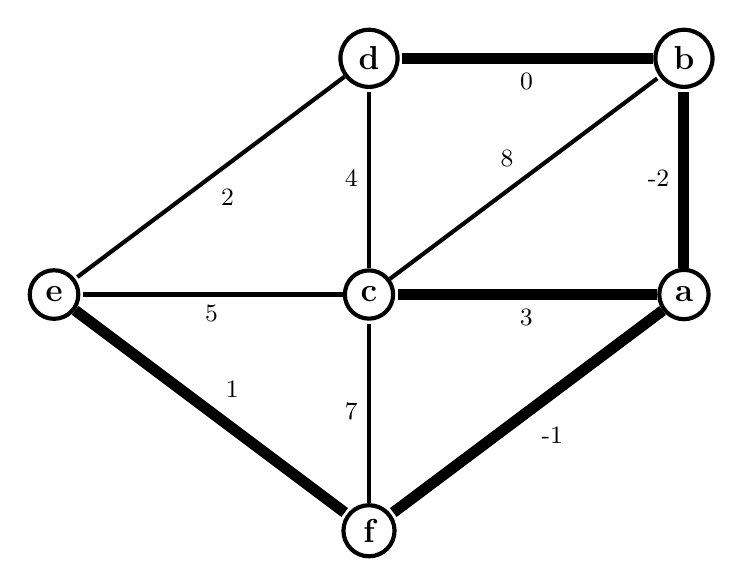
\begin{tikzpicture}[-,>=stealth,shorten >=1pt,auto,
    main node/.style={circle,draw,font=\large\bfseries}, line width=1.5pt]
  \node[main node] (a) at (-2,-1.5) {a};
  \node[main node] (b) at (-2,1.5) {b};
  \node[main node] (c) at (-6,-1.5) {c};
  \node[main node] (d) at (-6,1.5) {d};
  \node[main node] (e) at (-10,-1.5) {e};
  \node[main node] (f) at (-6,-4.5) {f};
  
  \path[every node/.style={font=\small}]
  (a) edge[line width=4pt] node {-2} (b) 
  edge[line width=4pt] node {3} (c)
  (b) edge[line width=4pt] node {0} (d)
  (a) edge[line width=4pt] node {-1} (f)
  (c) edge node {4} (d) 
  edge node {5} (e) 
  edge node {8} (b) 
  (d) edge node {2} (e)
  (e) edge[line width=4pt] node {1} (f) 
  (f) edge node {7} (c); 
  \end{tikzpicture}
\end{center}
I hvilken rækkefølge bliver kanterne inkluderet i det mindste udspændende træ når Kruskal's algoritme køres på denne graf? \etsvar
\mulighederstart
\svar \{a,b\}, \{a,c\}, \{a,f\}, \{b,d\}, \{e,f\}  % Lexicographically
\svar \{a,b\}, \{a,f\}, \{b,d\}, \{e,f\}, \{a,c\} \korrekt
\svar \{b,d\}, \{a,f\}, \{e,f\}, \{a,b\}, \{a,c\} % By absolute value
\svar \{b,d\}, \{a,c\}, \{e,f\}, \{a,b\}, \{a,f\} % Distractor
\svar \{b,d\}, \{a,f\}, \{e,f\}, \{a,b\}, \{a,c\}  % Distractor
\mulighederslut
\forklaring{Håndkørsel af Kruskal's algoritme og giver den angivne rækkefølge.}




\spoergsmaal{Korteste veje}
Betragt følgende orienterede, vægtede graf $G=(V,E)$:
\begin{center}
  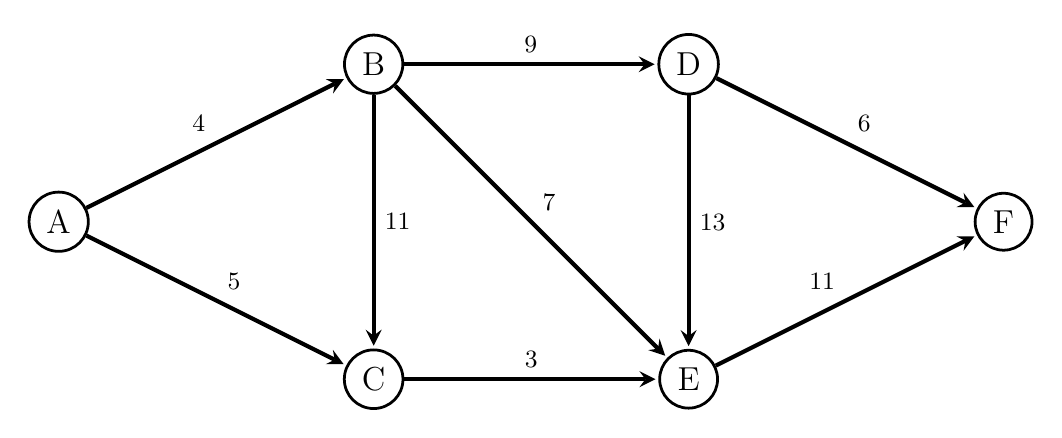
\begin{tikzpicture}[->,>=stealth,shorten >=1pt,auto,
      main node/.style={circle,draw,font=\large,line width=1pt}, line width=1.5pt]
  \node[main node] (a) at (0,0) {A};
  \node[main node] (b) at (4,2) {B};
  \node[main node] (c) at (4,-2) {C};
  \node[main node] (d) at (8,2) {D};
  \node[main node] (e) at (8,-2) {E};
  \node[main node] (f) at (12,0) {F};
  \path[every node/.style={font=\small}]
  (a) edge node {4} (b)
  (a) edge node {5} (c)
  (b) edge node {11} (c)
  (b) edge node {9} (d)
  (b) edge node {7} (e)
  (c) edge node {3} (e)
  (d) edge node {13} (e)
  (d) edge node {6} (f)
  (e) edge node {11} (f);
  \end{tikzpicture}
  \end{center}
Hvilke kanter er med i en korteste vej (eng.~\emph{shortest path}) fra knude A til \emph{mindst} én af knuderne \{B,C,D,E,F\}?
\fleresvar
\mulighederstart
\svar \{A,B\} \korrekt
\svar \{A,C\} \korrekt
\svar \{B,C\}
\svar \{B,D\} \korrekt
\svar \{B,E\}
\svar \{C,E\} \korrekt
\svar \{D,E\}
\svar \{D,F\} \korrekt
\svar \{E,F\} \korrekt
\mulighederslut
\forklaring{De fleste kanter på en korteste vej er i korteste-vej træet, der fx kan findes ved at håndkøre Dijkstra's algoritme. I det sidste skridt er der dog to mulige kanter til F der begge resulterer i en korteste vej, så de skal begge inkluderes.}





\spoergsmaal{Valg af algoritmer og datastrukturer}
Antag at du skal løse $k$-{\sc Difference} problemet, defineret således: Givet en parameter~$k$ og et array $A$ med $n$ heltal, afgør om der findes to tal i $A$ med en difference på $k$.

\medskip

\noindent
{\bf Eksempel.} Hvis $k=4$ og $A = \langle 2, 7, 13, 3, 11, 17\rangle$ er svaret ``ja'', fordi vi har $A[2]-A[4] = 7 - 3 = 4$. Hvis $k=3$ og $A$ er uændret er svaret ``nej'' da der ikke findes to tal i $A$ med en difference på 3.

\medskip

\noindent
Hvilken af følgende algoritmer og datastrukturer er mest relevant som en del af en simpel og effektiv algoritme, der løser $k$-{\sc Difference}?
\etsvar

\mulighederstart
\svar Dijkstra's algoritme
\svar Disjunkte mængder
\svar Dynamiske tabeller
\svar Merge-sort \korrekt
\svar Prim's algoritme
\mulighederslut
\forklaring{Ved først at sortere $A$ kan problemet løses i yderligere $O(n)$ tid ved at lave {\sc Merge} af $\langle A[1],\dots,A[n]\rangle$ og $\langle A[1]+k,\dots,A[n]+k\rangle$ og bemærke om der findes identiske elementer i de to lister. (Alternativt kan der laves $n$ binære søgninger efter et element med værdi $A[i]-k$, for $i=1,\dots,n$.) I begge tilfælde tager algoritmen totalt tid $O(n \lg n)$. De øvrige nævnte algoritmer og datastrukturer kan ikke umiddelbart bruges som en del af en simpel og effektiv algoritme.}




\multiplechoiceslut

\newpage


\section*{Skriftlige opgaver}\label{sec:written}

{\bf Skriftlige opgaver} afleveres som et Word dokument i ITX systemet.
Der er mulighed for at tegne og skrive på tablet, og indsætte i dokumentet.
\begin{itemize}
    \item Brug \emph{én side til hvert delspørgsmål, i samme rækkefølge som i opgavesættet.} 
    \item Delspørgsmålets nummer/bogstav (fx 19 eller 20.a) skal fremgå.
\end{itemize}





\section{Induktionsbeviser (7\%)}

Betragt følgende funktion, i pseudo-kode notationen fra CLRS, hvor input $A$ er et array af heltal, $n$ er længden af $A$, og $b$ er en heltalsparameter.
\begin{codebox}
  \Procname{$\proc{HeavyHitter}(A, n, b)$}
  \li let $r[1:b]$ be a new array
  \li \For $i = 1$ \To $b$
  \li \Do $r[i] = 0$ \End
  \li \For $j = 1$ \To $n$ \Do 
  \li \If $A[j]\geq 1$ and $A[j]\leq b$ \Do
  \li $r[A[j]] = r[A[j]] + 1$ \End \End
  \li \Return $\max_{1\leq\ell\leq b}(r[\ell])$
\end{codebox}

\noindent
{\bf Eksempel:} For $n=6$, $b=10$, $A = \langle 5,1,1,7,1,3\rangle$ returnerer {\sc HeavyHitter} værdien $3$.
\medskip

\punkt{a)}{ Forklar i ord hvad {\sc HeavyHitter} beregner.}

\forklaring{ {\sc HeavyHitter} beregner hvor mange gange det hyppigste element i $A$ forekommer, hvor elementer i $A$ der ikke ligger i intervallet $[1,\dots,b]$ ignoreres. }


\punkt{b)}{ Formulér en løkkeinvariant $I(j)$ der beskriver indholdet af $r$ efter iteration~$j$ af {\bf for}-løkken i linje 4--6.
Argumentér ved induktion for at invarianten gælder efter $j$ iterationer, for $j\geq 0$.
Invarianten $I(n)$, der gælder når løkken afsluttes skal underbygge dit svar i spørgsmål {\bf a)}.}

\forklaring{ Invariant $I(j)$: For $i\in\{1,\dots,b\}$ gælder $r[i] = |\{ k \; | \; 1\leq k \leq j \wedge A[k]=i \}|$.
Invarianten gælder for $j=0$ da $r[i]=0$ (pga.~initialiseringen i linje 2-3). 
I induktionsskridtet antager vi $I(j-1)$ og vil vise at $I(j)$ gælder efter iteration $j$.
Værdien af $r[i]$ øges med 1 i iteration $j$ præcis hvis $A[j]=i$, og det samme gælder for $|\{ k \; | \; 1\leq k \leq j \wedge A[k]=i \}|$.
}


\section{Så længe som muligt (12\%)}

Vi betragter følgende variant af problemet aktivitetsudvælgelse (eng.~\emph{activity selection}) fra CLRS sektion 15.1.
I stedet for at maksimere antallet af aktiviteter som i CLRS, vil vi vælge en mængde af aktiviteter, der samlet varer \emph{så lang tid som muligt}.
Vi er altså givet en mængde $S=\{a_1,a_2,\ldots,a_n\}$ af $n$ elementer, hvor hver aktivitet $a_i$ har en givet starttid $s_i$ og en sluttid $f_i$, så $0\leq s_i<f_i<\infty$.
Antag at aktiviterne er sorteret efter sluttider, dvs.~$f_1\leq f_2\leq\cdots\leq f_n$.
Vi ønsker at vælge en mængde $A\subseteq S$ af ikke-overlappende aktiviteter som maksimerer $\sum_{a_i\in A} (f_i-s_i)$.
At aktiviteterne i $A$ er ikke-overlappende vil sige at hvis $a_i,a_j\in A$ hvor $i\neq j$, så gælder $[s_i,f_i)\cap [s_j,f_j)=\emptyset$, dvs.~det er tilladt at $f_i = s_j$ eller $f_j = s_i$.

\punkt{a)}{
Antag at aktiviteterne er $S=\{a_1,a_2,a_3,a_4\}$ med starttider $s=\langle 0,3,1,6\rangle$ og sluttider $f=\langle 2,4,5,8\rangle$.
Angiv en optimal løsning $A$.}

\forklaring{Den optimale løsning er $\{a_3,a_4\}$, som har samlet varighed $6$.
\medskip}

For hvert $i\in\{0, 1,\ldots,n\}$, lad $S_i=\{a_1,a_2,\ldots,a_i\}$ være mængden bestående af de $i$ første aktiviteter, dvs.~$S_0=\emptyset$, $S_1=\{a_1\}$, $S_2=\{a_1, a_2\}$, osv.
Definér $t_i$ til at være den samlede tid for aktiviteterne i en optimal løsning til $S_i$, hvor specielt $t_0=0$.

\punkt{b)}{
  Betragt et fast indeks $i\in\{1,\ldots,n\}$ og lad $j\in\{0,1,\ldots,i-1\}$ være det største indeks hvor $f_j\leq s_i$ (her definerer vi $f_0=0$).
  Argumentér for at
\[
t_i=\max\{t_{i-1},t_j+f_i-s_i\}.
\]}

\forklaring{Enten inkluderer den optimale løsning til $S_i$ aktiviteten $a_i$, eller også gør den ikke.
I det første tilfælde skal vi udover $a_i$ vælge en optimal løsning blandt aktiviteter der slutter senest når $a_i$ starter, altså blandt $S_j$, hvor $j$ er defineret som i opgaveteksten.
I det andet tilfælde må løsningen være den samme som den optimale til $S_{i-1}$, altså $t_{i-1}$.
Dette viser at $t_i\leq \max\{t_{i-1},t_j+f_i-s_i\}$.
Begge de to kandidater er gyldige løsninger til $S_i$, så vi har også $t_i\geq \max\{t_{i-1},t_j+f_i-s_i\}$.
Derfor er $t_i=\max\{t_{i-1},t_j+f_i-s_i\}$.
}

\punkt{c)}{
Skriv pseudokode til en algoritme som returnerer den samlede tid $t_n$ af aktiviteterne i den optimale løsning til hele mængden $S$.
Signaturen på din pseudokode skal være
\[\textsc{Activity-Selection-Max-Span}(s,f,n),\]
hvor $s$ og $f$ er arrays af længde $n$ med hhv.~start- og sluttider.
For at få fuldt point skal algoritmen have køretid $O(n^2)$, men det er ikke nødvendigt at bevise grænsen for køretiden.}

\forklaring{Ifølge del b) kan vi bruge dynamisk programmering.
Her er en mulig løsning:

\medskip

\textsc{Activity-Selection-Max-Span}$(s,f,n)$

\quad Let $t[0:n]$ be a new array.

\quad $t[0]=0$

\quad for $i=1$ to $n$

\quad\quad Use binary search to find the max.~$j\in\{0,1,\ldots,i-1\}$ such that $j==0$ or $f[j]\leq s[i]$.

\quad\quad $t[i]=\max\{t[i-1],t[j]+f[i]-s[i]\}$

\quad return $t[n]$
}

\punkt{d)}{
Forklar hvordan man kan lave en algoritme som løser problemet i $O(n \lg n)$ tid.
Hvis din algoritme fra opgave c) allerede har denne køretid så argumentér for det.}

\forklaring{Algoritmen fra spørgsmål c) har køretid $O(n \lg n)$ fordi for-løkken itererer over $n$ værdier og vi bruger $O(\lg n)$ tid på binær søgning i hver iteration.}



\section{Så mange som muligt (9\%)}\label{sec:last}

Vi betragter et array af $n$ heltal $X=\langle x_1,x_2,\ldots,x_n\rangle$, hvor $x_i$ kan være positivt, negativt eller $0$.
Lad $S=\sum_{i=1}^n x_i$ være tallenes sum.
Vi ønsker at løse {\sc Longest-Subset-Sum} problemet: 
Find størrelsen på den største indeksmængde $I\subseteq \{1,2,\ldots, n\}$ hvor $\sum_{i\in I} x_i\leq S/2$.

\medskip
{\bf Eksempel.} For $X=\langle 1,4,2,8\rangle$, der har $S=15$, kan vi finde en mængde $I$ med~3 elementer, nemlig $I=\{1,2,3\}$. Dette er den størst mulige mængde der overholder $\sum_{i\in I} x_i\leq S/2$ for ingen løsning kan indeholde alle fire elementer.


\punkt{a)}{Giv et eksempel på et array $X$ hvor løsningen ikke er entydig, dvs.~hvor der findes to \emph{forskellige} indeksmængder $I_1$ og $I_2$ af højst mulige størrelse hvor $\sum_{i\in I_1} x_i\leq S/2$ og $\sum_{i\in I_2} x_i\leq S/2$.}

\forklaring{Eksempel: $X=\langle 1,1\rangle$ har to optimale løsninger: $I=\{1\}$ og $I=\{2\}$, begge af størrelse 1. }

\medskip

Vi ser nu på følgende tilgang til at løse {\sc Longest-Subset-Sum}: Start med summen af alle tal i~$X$ og fjern ét tal ad gangen i omvendt sorteret rækkefølge så længe summen er højere end~$S/2$. Returnér antallet af elementer, der ikke er fjernet fra $X$.

\medskip
{\bf Eksempel.} For $X=\langle 4, -2, -3, 2, 5, 5\rangle$, der har sum $S=11$, fjerner vi de to største elementer $5$ og $5$, hvorefter summen af de fire resterende tal er 1, hvilket er mindre end eller lig med $S/2$. Derfor returneres 4.

\punkt{b)}{
Bevis at en optimal løsning til {\sc Longest-Subset-Sum} kan konstrueres som beskrevet ovenfor.}

\forklaring{
Antag at $X$ er sorteret i ikke-faldende rækkefølge, så den foreslåede algoritme vil fjerne tallene fra summen i rækkefølgen $x_n,x_{n-1},\ldots,x_1$.
Betragt en vilkårlig indeksmængde $I^*\subseteq \{1,2,\ldots, n\}$ som giver en optimal løsning, og lad $k=\mid I^*\mid$ være antallet af tal i $I^*$ og lad $I=\{1,2,\ldots,k\}$.
Hvis ikke $I^*=I$, så giver $I$ en sum som er højst så stor som den for $I^*$, så $I$ er også en optimal indeksmængde.
Siden $I$ er optimal, har vi $\sum_{i=1}^{k'} x_i>S/2$ for ethvert $k'\in\{k+1,\ldots,n\}$.
Derfor finder den foreslåede algoritme det optimale antal $k$.}

\punkt{c)}{Skriv pseudokode til en algoritme der løser {\sc Longest-Subset-Sum}.
Signaturen til din algoritme skal være \[\textsc{Longest-Subset-Sum}(x,n),\]
hvor $x$ er et array af længde $n$.}

\forklaring{Ifølge del b) giver en simpel grådig algoritme en optimal løsning. Pseudo-koden kan fx se således ud:

\textsc{Longest-Subset-Sum}$(x,n)$

\quad Sort $x$ in non-decreasing order, for instance using \textsc{Merge-Sort}.

\quad Let $S$ be the sum of the numbers in $x$.

\quad $R=S$

\quad $i=n$

\quad while $R>S/2$

\quad\quad $R = R - x[i]$

\quad\quad $i=i-1$

\quad return $i$
}



\label{page:last}
